\documentclass[11pt,a4paper]{article}
% Preámbulo común de los informes de docs/reports/ (no forma parte de la memoria).
\usepackage[T1]{fontenc}
\usepackage[utf8]{inputenc}
\usepackage[spanish,es-noshorthands,es-tabla]{babel}
\usepackage{lmodern}
\usepackage{microtype}
\usepackage[a4paper,margin=2.3cm]{geometry}
\usepackage{graphicx}
\usepackage{booktabs}
\usepackage{tabularx}
\usepackage{array}
\usepackage{multirow}
\usepackage{amsmath}
\usepackage{enumitem}
\usepackage{float}
\usepackage{adjustbox}
\newcommand{\fittable}[1]{\begin{adjustbox}{max width=\linewidth}\input{#1}\end{adjustbox}}
\usepackage[font=small,labelfont=bf]{caption}
\usepackage[dvipsnames,table]{xcolor}
\usepackage{fancyhdr}
\usepackage[most]{tcolorbox}
\usepackage[hidelinks]{hyperref}

\definecolor{accent}{HTML}{2A78D6}
\definecolor{inkmuted}{HTML}{52514E}
\definecolor{boxbg}{HTML}{F3F6FB}
\definecolor{warnbg}{HTML}{FDF6E7}
\definecolor{warnline}{HTML}{C98500}

\setlist{itemsep=2pt,topsep=4pt}
\setlength{\parindent}{0pt}
\setlength{\parskip}{5pt}
\renewcommand{\arraystretch}{1.12}

\newtcolorbox{keybox}[1][]{colback=boxbg,colframe=accent,boxrule=0.6pt,arc=2pt,
  left=8pt,right=8pt,top=6pt,bottom=6pt,fonttitle=\bfseries,title={#1}}
\newtcolorbox{warnbox}[1][]{colback=warnbg,colframe=warnline,boxrule=0.6pt,arc=2pt,
  left=8pt,right=8pt,top=6pt,bottom=6pt,fonttitle=\bfseries,title={#1}}

\newcommand{\estado}[1]{\textsf{\small\textbf{\color{accent}#1}}}
\newcommand{\ruta}[1]{\texttt{\small #1}}

\pagestyle{fancy}
\fancyhf{}
\renewcommand{\headrulewidth}{0.3pt}
\fancyfoot[C]{\small\color{inkmuted}\thepage}

\fancyhead[L]{\small\color{inkmuted}QCNN variacional: resultados experimentales}
\fancyhead[R]{\small\color{inkmuted}12 de noviembre de 2026}
\graphicspath{{figures/}}

\title{\textbf{Línea variacional de la QCNN}\\[2pt]\large Resultados experimentales de las fases A, B y C}
\author{TFG «Plataforma para la experimentación con Quantum Machine Learning»}
\date{12 de noviembre de 2026 · revisión \texttt{bc877bd} + cambios posteriores (commits \texttt{dec0f0b}--\texttt{4424eb7})}

\begin{document}
\maketitle
\thispagestyle{fancy}

\begin{keybox}[Resumen]
\textbf{Estado: evaluado en simulación} (CPU, sin QPU). Todas las cifras y figuras se derivan de los JSON
persistidos en \ruta{results/variational/} mediante \ruta{experiments/plot\_variational\_report.py}.
\begin{enumerate}[leftmargin=*]
  \item La QCNN de 4 qubits \textbf{aprende}: supera con claridad a la clase mayoritaria en ambos datasets.
  \item \textbf{Queda por debajo de una regresión logística} con las mismas 4 características. En 10 particiones
        nuevas la diferencia es de $-0{,}026$ a $-0{,}084$ en Breast Cancer y de $-0{,}07$ a $-0{,}18$ en Iris.
  \item \textbf{No hay un optimizador mejor en accuracy}: frente a Adam, ninguna diferencia es significativa tras la
        corrección de Holm. Las diferencias vistas en una única partición (fase B) no se replican.
  \item \textbf{El optimizador secuencial es mucho más barato}: llega a su mejor checkpoint con 3,2--9,4 veces menos
        circuitos que Adam, en las 40 combinaciones de partición, dataset y codificación.
  \item La \textbf{codificación angular} es, en media, mejor que la de fase en ambos datasets.
\end{enumerate}
\end{keybox}

\begin{warnbox}[Nota posterior (24 de noviembre): el circuito solo usa 3 características y 5 pesos]
Un diagnóstico posterior (\ruta{results/diagnostics/light-cone/}; log, sección 37) muestra que la salida de este
circuito no depende de la cuarta característica ni de los pesos $w_1$--$w_3$ de la segunda capa. Dos CNOT idénticas
entre convolución y pooling se anulan. Las cifras de este informe son válidas para este circuito, pero describen un
modelo con 3 características y 5 parámetros efectivos. Corregir la arquitectura es una decisión pendiente.
\end{warnbox}

\section{Modelo y protocolo}

\subsection{Modelo}
QCNN de 4 qubits implementada en Qibo y reproducida por un simulador NumPy vectorizado
(\ruta{src/fast\_qcnn.py}) que coincide con Qibo con error $<10^{-10}$. Cada muestra, con 4 características
normalizadas en $[0,1]$, se codifica de dos formas:
\begin{itemize}
  \item \textbf{angular}: $R_Y(\pi x)$ sobre cada qubit;
  \item \textbf{fase}: $H$ seguida de $R_Z(2\pi x)$.
\end{itemize}
Siguen dos capas de filtros convolucionales compartidos con \textit{pooling} lógico. El modelo tiene 8 pesos
(forma $2\times 4$): cada peso de la primera capa aparece 3 veces en el circuito y cada peso de la segunda, una.
La salida es el valor esperado de $Z$ en el qubit superviviente, y la pérdida, el error cuadrático frente a
etiquetas $\pm 1$.

\subsection{Optimizadores}
Todos siguen el modelo de ejecución estándar en hardware actual: el circuito calcula valores esperados y un
optimizador clásico actualiza los pesos.
\begin{itemize}
  \item \textbf{GD}: descenso de gradiente con gradiente exacto por \textit{parameter-shift} (2 evaluaciones por
        aparición de cada peso).
  \item \textbf{Adam}: el mismo gradiente con momentos adaptativos de primer y segundo orden.
  \item \textbf{SPSA}: estima el gradiente con solo 2 evaluaciones por paso, perturbando todos los pesos a la vez en
        una dirección aleatoria, con ganancias decrecientes.
  \item \textbf{Secuencial} (tipo Rotosolve/NFT): recorre los pesos uno a uno. Como el coste es un polinomio
        trigonométrico de cada peso, lo reconstruye exactamente con $2R+1$ evaluaciones ($R$ = número de apariciones)
        y salta a su mínimo, que se busca en una rejilla de 2048 puntos. No tiene tasa de aprendizaje.
        \textit{Las referencias de Rotosolve/NFT aún no están verificadas en \ruta{memory/bibliography.bib}.}
\end{itemize}

\begin{table}[H]
\centering\small
\caption{Coste por paso de optimización, en ejecuciones del circuito. Los totales usan 398 (Breast Cancer) y 70 (Iris)
muestras de entrenamiento.}
\begin{tabular}{lrrr}
\toprule
Optimizador & Por muestra y paso & Breast Cancer & Iris \\
\midrule
GD / Adam  & $33 = 1 + 2(4\cdot 3 + 4\cdot 1)$ & 13\,134 & 2\,310 \\
SPSA       & $2$                               & 796     & 140 \\
Secuencial & $40 = 4\cdot 7 + 4\cdot 3$         & 15\,920 & 2\,800 \\
\bottomrule
\end{tabular}
\end{table}

\subsection{Protocolo común}
\begin{itemize}
  \item Partición estratificada 70/15/15; la normalización y el PCA (Breast Cancer, 4 componentes) se ajustan solo con train.
  \item Checkpoint por \textbf{mínima pérdida de validation}, incluido el paso 0. \textbf{Test se evalúa una sola vez},
        después de elegir el checkpoint, y nunca se usa para seleccionar nada.
  \item Baselines evaluadas en test: clase mayoritaria y regresión logística sobre las mismas características.
  \item Estadística: IC95\,\% bootstrap (10\,000 remuestreos), Wilcoxon de rangos con signo y corrección de Holm donde se indica.
  \item Semillas separadas: partición (dataset), inicialización de pesos (8 semillas: 19--47) y ejecución (101).
\end{itemize}

\begin{table}[H]
\centering\small
\caption{Fases del benchmark.}
\begin{tabularx}{\linewidth}{lXl}
\toprule
Fase & Qué se hizo & Fuente \\
\midrule
A & Ajuste de hiperparámetros solo con validation. Breast Cancer, partición 42, 3 semillas, 60 pasos. & \ruta{A-tuning-bc-exact/} \\
B & Confirmación en la partición 42 con 8 semillas nuevas y test una vez, en 4 condiciones: exacta, 1000 shots,
    shots con ruido ($p=0{,}001$ y lectura 2\,\%) y mismo presupuesto de circuitos. Breast Cancer e Iris. & \ruta{B-confirm-bc/}, \ruta{B-confirm-iris/} \\
C & Robustez frente a la partición: 10 particiones nuevas por dataset, simulación exacta, 1280 entrenamientos.
    Pre-registrada. & \ruta{C-partitions/} \\
\bottomrule
\end{tabularx}
\end{table}

\section{Fase A: ajuste de hiperparámetros}

\begin{figure}[H]
\centering
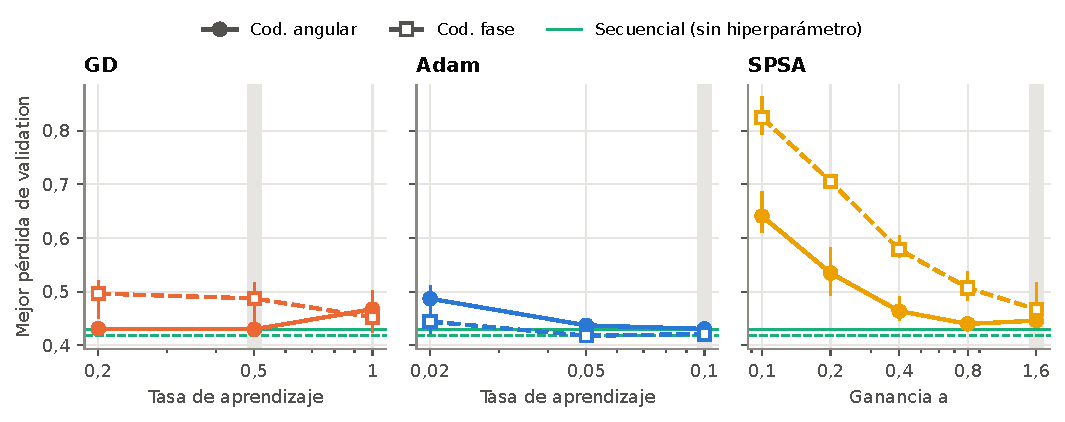
\includegraphics[width=\linewidth]{fig01_phaseA_tuning.pdf}
\caption{Mejor pérdida de validation frente al hiperparámetro (media de 3 semillas; barras: mínimo y máximo).
Las líneas verdes son el secuencial, que no tiene hiperparámetro. La banda gris marca el valor elegido.
Breast Cancer, partición 42, 60 pasos, sin test.}
\end{figure}

La regla, fijada antes de ejecutar, fue elegir por optimizador el valor con menor pérdida media de validation,
promediando ambas codificaciones. Se eligieron GD con $\mathit{lr}=0{,}5$, Adam con $\mathit{lr}=0{,}1$ y SPSA con
$a=1{,}6$ ($c=0{,}1$, $A=6$).
\begin{itemize}
  \item \textbf{GD y Adam} son poco sensibles en el rango probado: las diferencias entre los dos mejores valores caben en
        la variación entre semillas.
  \item \textbf{SPSA} depende mucho de la ganancia $a$. Su óptimo quedó en el borde de la rejilla incluso tras ampliarla,
        lo que indica que con 60--100 pasos está limitado por el número de pasos.
  \item \textbf{El secuencial} alcanza, sin ajuste, la misma pérdida que los mejores GD y Adam.
\end{itemize}

\section{Fase B: confirmación en una partición}

\begin{figure}[H]
\centering
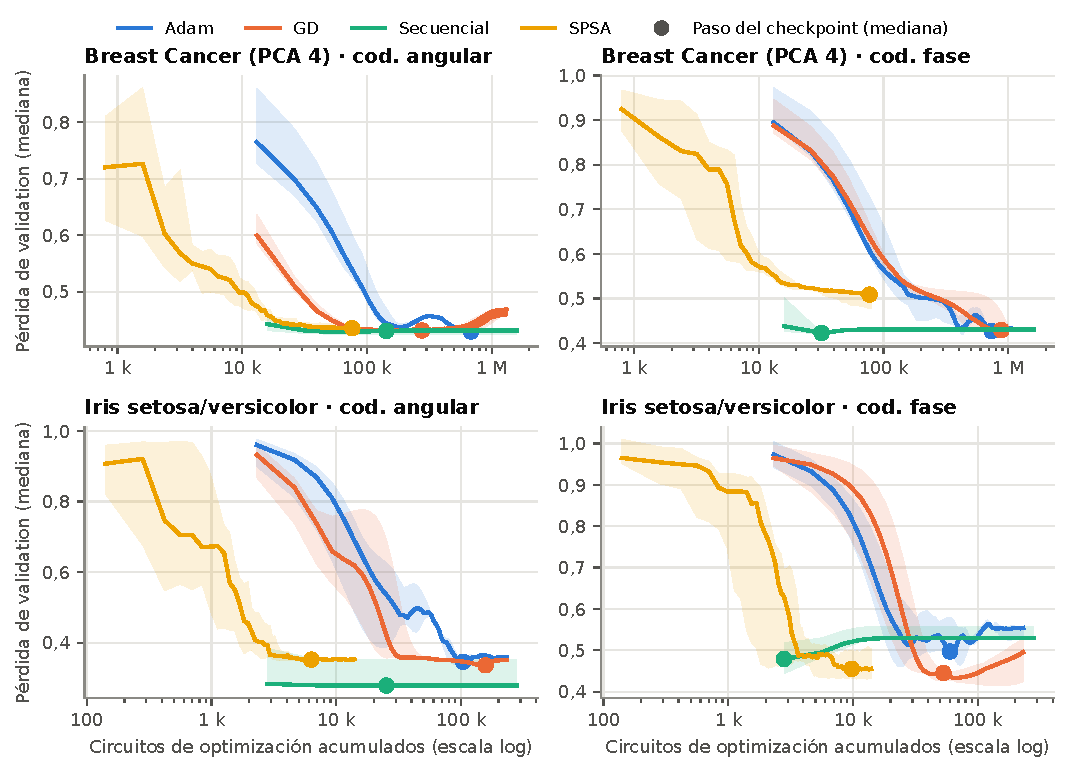
\includegraphics[width=\linewidth]{fig02_phaseB_curves.pdf}
\caption{Pérdida de validation frente a los circuitos de optimización acumulados (escala logarítmica; mediana de
8 semillas y banda intercuartílica). El punto marca el paso mediano del checkpoint. Partición 42, simulación exacta.}
\end{figure}

La figura muestra el coste real de cada optimizador:
\begin{itemize}
  \item \textbf{SPSA} es el más barato por paso, pero en codificación de fase sobre Breast Cancer se estanca en una
        pérdida más alta (unos 0,51) dentro de los 100 pasos.
  \item \textbf{El secuencial} parte de la mejor posición: tras el primer barrido ya está cerca de su mínimo.
  \item \textbf{GD y Adam} necesitan del orden de $10^5$ circuitos para llegar a la misma pérdida, y su checkpoint suele
        caer mucho más tarde por mejoras pequeñas.
  \item En Iris con codificación de fase la pérdida de validation del secuencial sube después del mínimo. Es un
        sobreajuste que la selección por validation controla.
\end{itemize}

\begin{figure}[H]
\centering
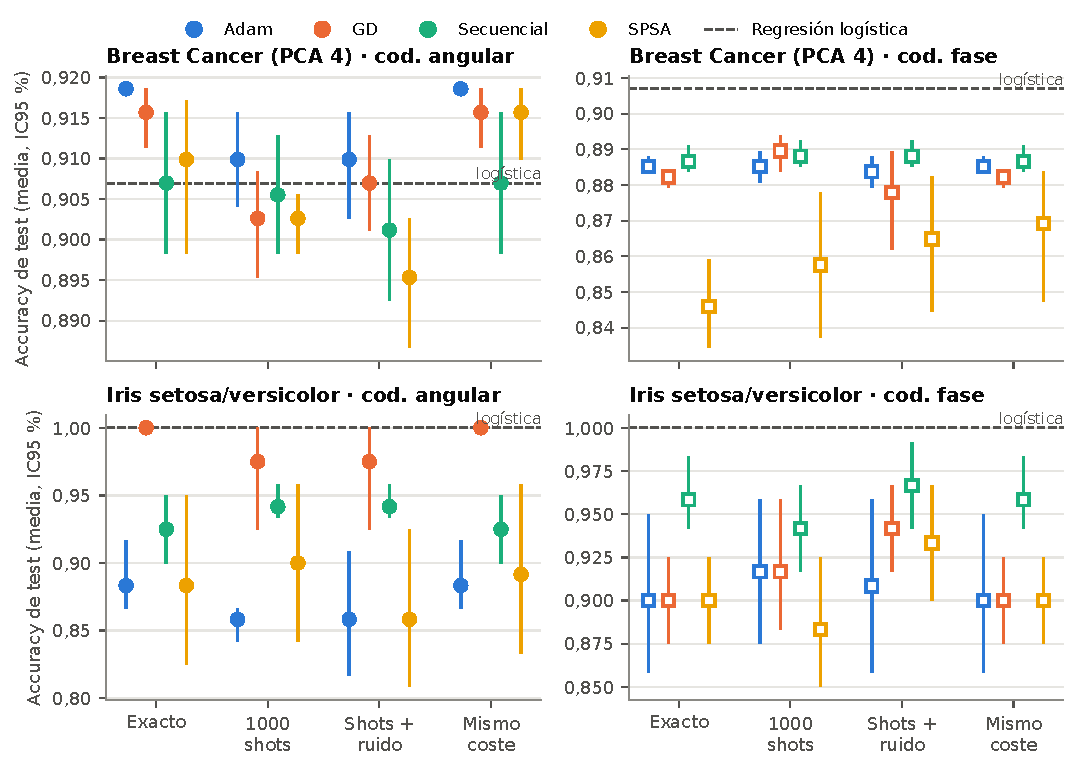
\includegraphics[width=\linewidth]{fig03_phaseB_conditions.pdf}
\caption{Accuracy de test por condición de ejecución (media de 8 semillas; IC95\,\% bootstrap). Partición 42.
La clase mayoritaria (0,628 en Breast Cancer, 0,467 en Iris) queda fuera de escala.}
\end{figure}

\begin{table}[H]
\centering\small
\caption{Accuracy de test media (8 semillas) por condición en la partición 42.}
\fittable{tables/tab_phaseB_accuracy}
\end{table}

Lectura de la fase B (una sola partición, sin corrección por multiplicidad):
\begin{itemize}
  \item \textbf{Shots y ruido} apenas cambian la accuracy. El ruido de sensibilidad no es una calibración de hardware.
  \item En Breast Cancer, Adam angular (0,919) supera a la logística (0,907); en fase, todos quedan por debajo.
  \item En Iris, GD angular acierta los 15 casos de test con las 8 semillas, mientras Adam se queda en 0,88.
        \textbf{La fase C muestra que ambas observaciones eran propias de la partición 42.}
\end{itemize}

\section{Fase C: robustez frente a la partición}

Diseño pre-registrado antes de ejecutar (\ruta{results/variational/C-partitions/README.md}):
\begin{itemize}
  \item 10 particiones nuevas por dataset (semillas 1--10), 4 optimizadores, 2 codificaciones y 8 semillas: 1280 entrenamientos.
  \item Hiperparámetros de la fase A, sin reajuste. La partición 42 queda fuera del análisis principal porque sirvió para el ajuste.
  \item \textbf{La unidad de análisis es la partición}: primero se promedian las 8 semillas dentro de cada partición y
        después se analizan las 10 particiones.
\end{itemize}

\subsection{Accuracy de test}

\begin{figure}[H]
\centering
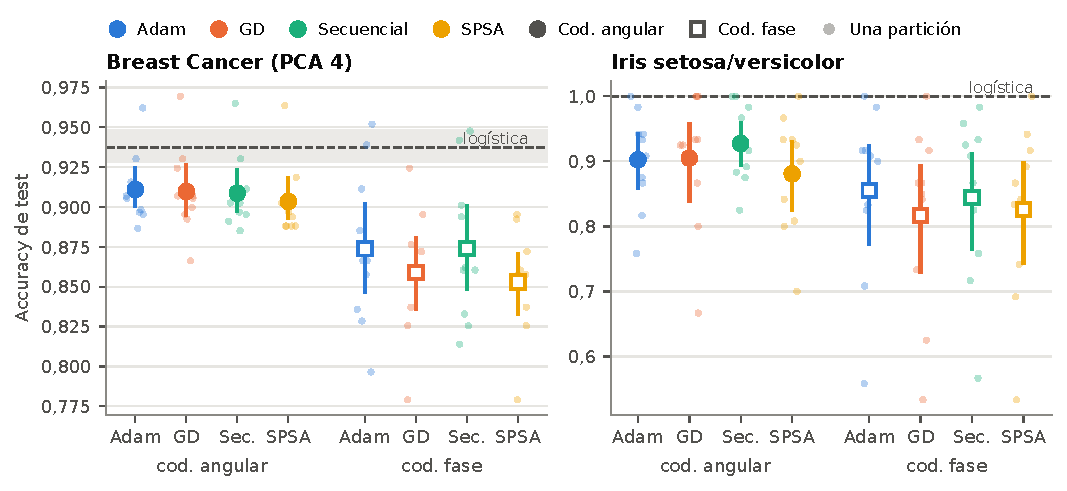
\includegraphics[width=\linewidth]{fig04_phaseC_accuracy.pdf}
\caption{Accuracy de test en 10 particiones. Los puntos pequeños son la media de cada partición; el marcador grande,
la media con su IC95\,\% sobre particiones. La línea discontinua es la regresión logística (banda: IC95\,\%).}
\end{figure}

\begin{table}[H]
\centering\scriptsize
\caption{Resumen de la fase C (media $\pm$ sd sobre 10 particiones). La diferencia frente a Adam se calcula por
partición; Holm se aplica dentro de cada dataset sobre las 6 comparaciones.}
\fittable{tables/tab_phaseC_summary}
\end{table}

\begin{figure}[H]
\centering
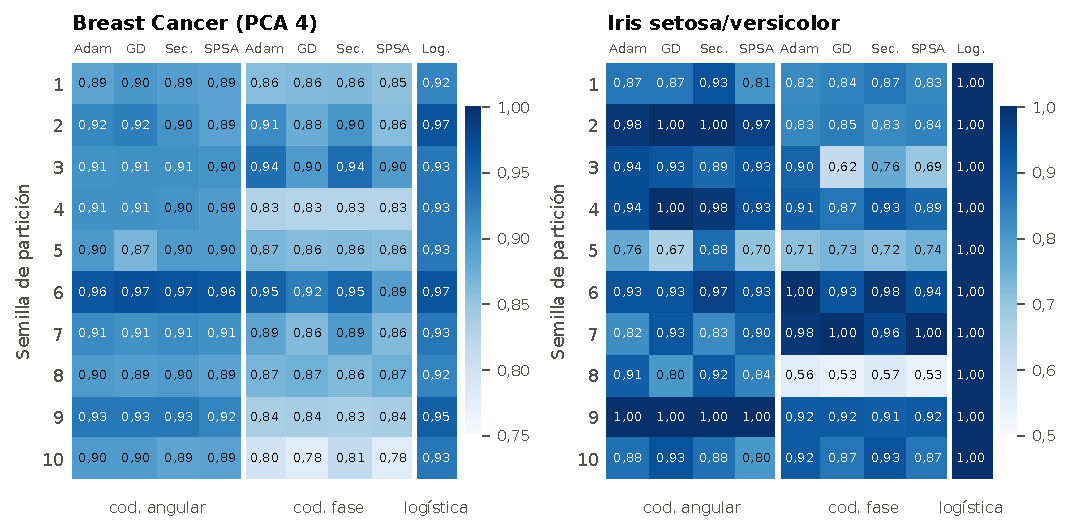
\includegraphics[width=\linewidth]{fig05_phaseC_partition_heatmap.pdf}
\caption{Accuracy de test por partición (filas) y condición (columnas; media de 8 semillas). Las filas varían mucho
más que las columnas: \textbf{la partición pesa más que el optimizador}.}
\end{figure}

El mapa de calor es la clave de esta fase:
\begin{itemize}
  \item En Iris, la misma QCNN pasa de 0,53--0,57 (partición 8, fase) a 1,00 (partición 9, angular) solo por cambiar la partición.
  \item Dentro de una fila, los cuatro optimizadores suelen quedar muy cerca.
  \item La regresión logística acierta los 15 casos de test de Iris en las 10 particiones.
\end{itemize}

\subsection{Comparación entre optimizadores}

\begin{figure}[H]
\centering
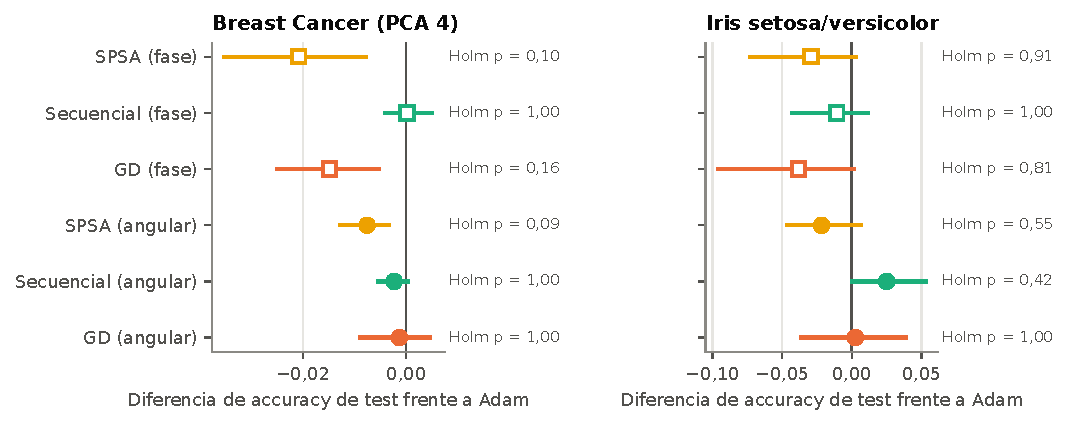
\includegraphics[width=\linewidth]{fig06_phaseC_forest_vs_adam.pdf}
\caption{Diferencia de accuracy de test frente a Adam, por partición (media e IC95\,\% bootstrap sobre 10 particiones),
con la $p$ de Wilcoxon corregida por Holm.}
\end{figure}

\begin{itemize}
  \item \textbf{Ninguna diferencia es significativa tras Holm.}
  \item En Breast Cancer, SPSA queda por debajo de Adam en ambas codificaciones con un IC que excluye el cero
        (sin corregir, $p\approx 0{,}02$), pero tras Holm $p\approx 0{,}09$--$0{,}10$.
  \item En Iris todos los IC cruzan el cero.
\end{itemize}

\begin{table}[H]
\centering\scriptsize
\caption{Observaciones de la fase B comprobadas en la fase C (pre-registradas; Holm sobre el bloque de 7 contrastes).
La columna $+/-$ indica en cuántas particiones la diferencia es positiva o negativa.}
\fittable{tables/tab_phaseC_observations}
\end{table}

\begin{itemize}
  \item \textbf{O1 no se replica}: la ventaja de GD sobre Adam en Iris era de la partición 42.
  \item \textbf{O2 y O3} mantienen la dirección (SPSA en fase peor que Adam; angular mejor que fase), pero no superan Holm.
        Al añadir la partición 42 quedan en Holm $p=0{,}029$ y $0{,}049$; no es el análisis principal, porque esa
        partición se usó para ajustar.
  \item \textbf{O4 se replica} en las 40 combinaciones: el secuencial siempre necesita menos circuitos.
\end{itemize}

\subsection{Coste frente a accuracy}

\begin{figure}[H]
\centering
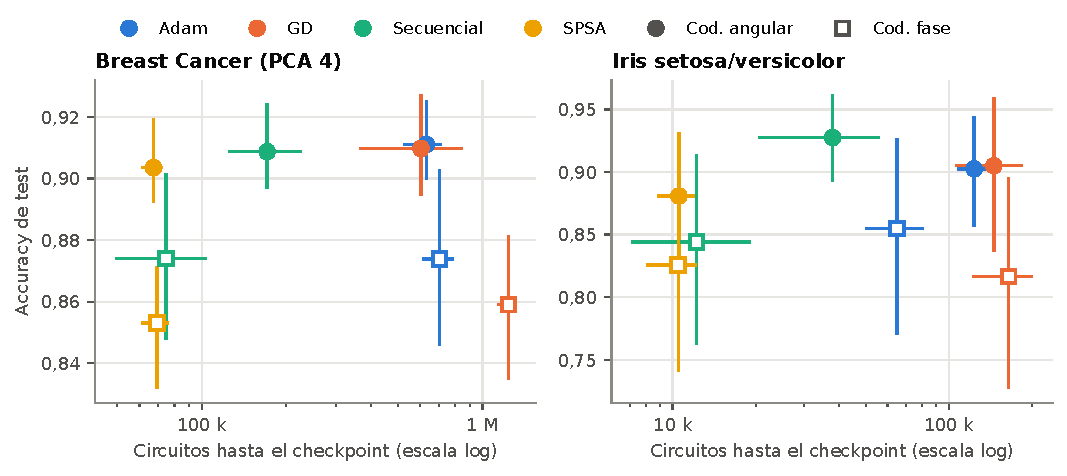
\includegraphics[width=\linewidth]{fig07_phaseC_cost_accuracy.pdf}
\caption{Circuitos de optimización hasta el checkpoint frente a la accuracy de test (medias con IC95\,\% sobre particiones).}
\end{figure}

\begin{itemize}
  \item \textbf{El secuencial} logra la misma accuracy que Adam y GD con 3,2--9,4 veces menos circuitos hasta su checkpoint
        (razón de medias).
  \item \textbf{SPSA} es el más barato en circuitos, pero tiende a quedar algo por debajo en accuracy, sobre todo en fase.
  \item \textbf{GD en fase} es el más caro: su checkpoint suele estar cerca del último paso.
\end{itemize}
Esto importa para hardware, donde el coste se mide en ejecuciones del circuito.

\subsection{Distancia a la regresión logística}

\begin{table}[H]
\centering\scriptsize
\caption{QCNN $-$ regresión logística en accuracy de test, por partición.}
\fittable{tables/tab_phaseC_gap_logistic}
\end{table}

\begin{itemize}
  \item La QCNN queda \textbf{por debajo de la logística en todos los casos}, con IC que excluyen el cero.
  \item Por condición, como mucho 1 de 10 particiones alcanza a la logística en Breast Cancer, y 3 de 10 en Iris.
  \item La conclusión de la fase B, «a la altura de la logística», era optimista: la partición 42 favorecía a la QCNN.
\end{itemize}

\subsection{Parada temprana (patience)}

En simulación exacta, el entrenamiento con \textit{patience} $P$ equivale exactamente a truncar el historial de
100 pasos en el primer paso con $P$ pasos sin mejora de validation. Una prueba unitaria lo verifica frente a
entrenamientos reales. La accuracy de test del checkpoint truncado se evaluó una vez por regla y no se usó para
elegir $P$.

\begin{figure}[H]
\centering
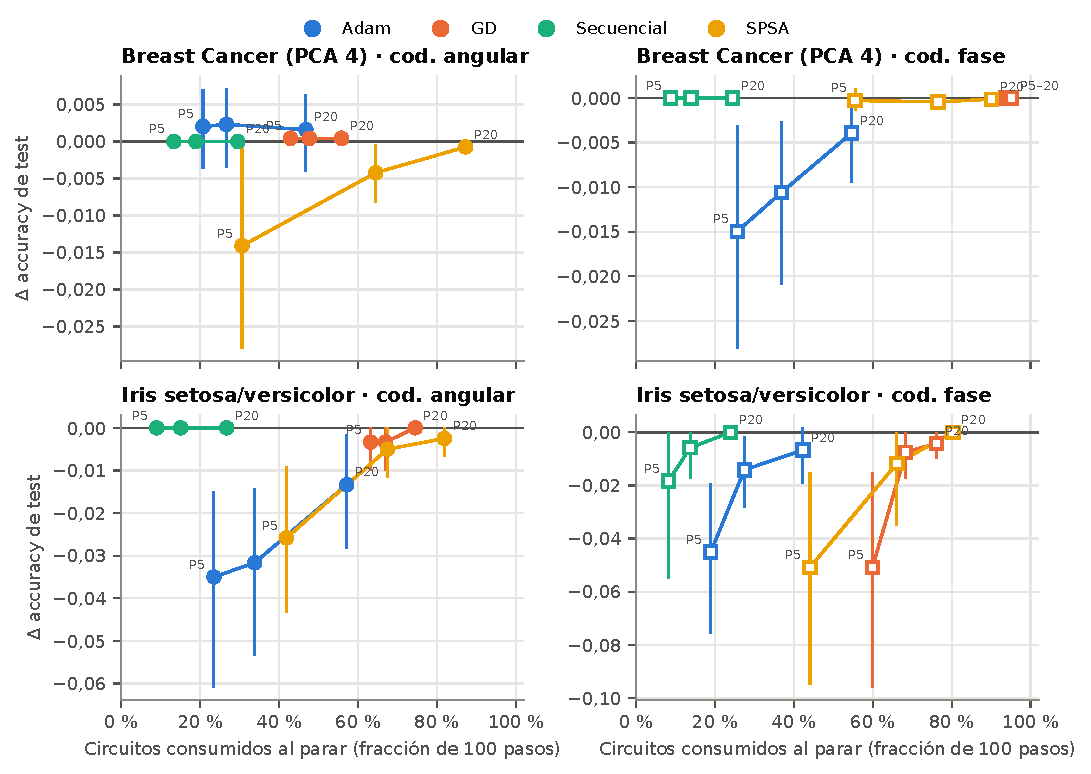
\includegraphics[width=\linewidth]{fig08_phaseC_patience.pdf}
\caption{Circuitos consumidos al parar (fracción de los de 100 pasos) frente a la pérdida de accuracy de test
respecto al checkpoint de 100 pasos, para $P=5$, 10 y 20 (de izquierda a derecha en cada línea). Media e IC95\,\%
sobre particiones.}
\end{figure}

\begin{table}[H]
\centering\scriptsize
\caption{Patience $P=10$: fracción de entrenamientos que paran antes de 100 pasos, fracción con el mismo checkpoint,
circuitos consumidos y cambio en accuracy de test (medias sobre particiones).}
\fittable{tables/tab_phaseC_patience10}
\end{table}

\begin{itemize}
  \item \textbf{Secuencial}: para con el 8--30\,\% de sus circuitos sin perder accuracy (con $P\ge 10$, cambio $\ge -0{,}006$).
  \item \textbf{Adam}: casi siempre para antes de 100 pasos, pero con $P$ pequeña pierde accuracy (hasta $-0{,}045$ en Iris con $P=5$).
  \item \textbf{SPSA} necesita $P$ grande.
  \item \textbf{GD} apenas para antes en Breast Cancer con codificación de fase.
\end{itemize}
Con la misma regla $P=10$ para todos, el secuencial consume entre 1,2 y 2,2 veces menos circuitos que Adam hasta
parar. Es una ventaja menor que la de O4, porque aquí se cuenta también lo que cuesta detectar la parada.

\section{Conclusiones y limitaciones}

\begin{keybox}[Qué se puede afirmar]
\begin{enumerate}[leftmargin=*]
  \item La QCNN variacional aprende ambos problemas: supera a la clase mayoritaria en todas las particiones.
  \item Con las mismas 4 características de entrada, \textbf{no alcanza a una regresión logística}. La salida del
        circuito solo depende de 3 de ellas (nota del 24 de noviembre).
  \item \textbf{El orden de los optimizadores en accuracy depende de la partición}; no hay diferencias significativas tras Holm.
  \item \textbf{El hallazgo robusto es de coste}: el optimizador secuencial reduce las ejecuciones del circuito sin perder accuracy.
\end{enumerate}
\end{keybox}

\begin{warnbox}[Limitaciones]
\begin{itemize}[leftmargin=*]
  \item Solo simulación en CPU. El ruido ($p=0{,}001$, lectura 2\,\%) es de sensibilidad, no una calibración, y solo se
        midió en la partición 42. No hay ejecución en QPU.
  \item Las particiones comparten muestras: la variación entre ellas mide la sensibilidad a la partición, no la
        incertidumbre frente a datos nuevos.
  \item Iris tiene 15 casos de test por partición (un caso equivale a 6,7 puntos).
  \item Los hiperparámetros se ajustaron en la partición 42 de Breast Cancer y se transfirieron a Iris.
  \item Wilcoxon con $n=10$ tiene una $p$ mínima de 0,002; la potencia es limitada.
  \item Estos resultados son de la línea variacional. \textbf{La ruta QGD no está evaluada}: ninguna ejecución QGD ha movido los pesos.
\end{itemize}
\end{warnbox}

\section{Reproducibilidad}

\begin{itemize}
  \item Las 160 invocaciones de la fase C terminaron con \texttt{EXIT\_CODE=0}. Cada \ruta{manifest.json} guarda la
        revisión Git, el hash del diff, los hashes del código no versionado, las versiones de los paquetes, el comando y
        las huellas de las particiones.
  \item Análisis de las fases A y B: \ruta{experiments/analyze\_variational\_benchmark.py}.
  \item Análisis de la fase C: \ruta{experiments/analyze\_partitions.py}, que reproduce las métricas de test
        almacenadas con error 0.
  \item Figuras y tablas de este informe:\\
        \ruta{qml\_env/Scripts/python.exe -B -m experiments.plot\_variational\_report}
  \item Detalle y desviaciones: \ruta{docs/TFG-technical-log.md} (secciones 30--34) y los README de cada fase.
\end{itemize}

\end{document}
